\begin{theorem} (Структура открытых множеств в $\R^n$)
	Каждое открытое множество в $\R^n$ представимо не более чем счётным объединением непересекающихся брусьев
\end{theorem}

\begin{proof}
	Для начала заметим, что мы можем записать $\R^n$ следующим образом:
	\[
		\R^n = \bigsqcup_{\vv{m} \in \Z^n} \prod_{i = 1}^n \left[\frac{m_i}{2^k}; \frac{m_i + 1}{2^k}\right),\ \ k \in \N_0
	\]
	где понятно, что $\vv{m} = (m_1, \ldots, m_n)$. Обозначим каждый брусок в этом представлении через $P_{\vv{m}, k}$. Теперь, рассмотрим произвольное открытое множество $G$. Введём следующее множество:
	\[
		M_0 = \bigsqcup_{\vv{l} \colon P_{\vv{l}, 0} \subset G} P_{\vv{l}, 0}
	\]
	Аналогично будем строить $M_m$, но с небольшим нюансом:
	\[
		M_m = \left(\bigsqcup_{\vv{l} \colon P_{\vv{l}, m} \subset G} P_{\vv{l}, m}\right) \bs \bigsqcup_{j = 0}^{m - 1} M_j
	\]
	По построению получили, что все $M_m$ не пересекаются.
	
	Идея тут состоит в том, что мы сначала рассекаем $\R^n$ сеткой с шагом $1$, берём все кубики попавшие внутри множества, потом делаем сетку плотнее в два раза, и у нас появляются ещё кубики поменьше, которые мы не взяли ранее, но они внутри множества, возьмём и их и т.д. (см. картинку).
	\\
	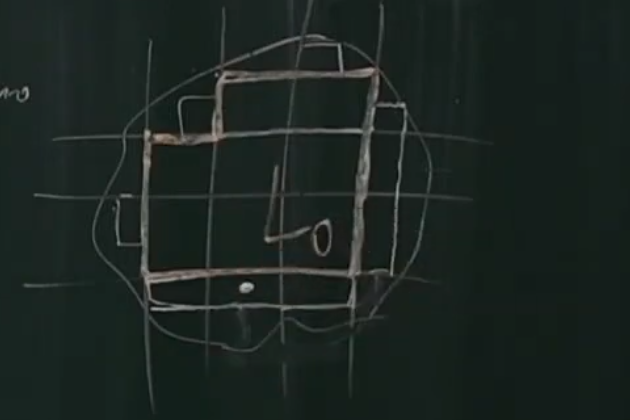
\includegraphics[width=0.7\textwidth]{images/th_5.3.8_open_set.png}
	\\
	Остаётся показать следующий факт:
	\[
		G = \bigsqcup_{m = 0}^\infty M_m
	\]
	По построению сразу верно включение $\supset$. Чтобы доказать в другую сторону, нам поможет свойство открытости $G$. 
	
	Рассмотрим $(\forall x \in G)$. Тогда $(\exists r > 0) : U_r(x) \subset G$ и более того, довольно очевидно, что выполнится следующее условие (как минимум из тех соображений, что мы можем делать сетку сколь угодно малой (достаточно чтобы диаметр кубика сетки был меньше чем радиус окрестности) и найти точку рядом с $x$):
	\[
		(\exists m_0\in\N_0)\ (\exists \vv{l}\in\Z^n) : x \in \prod_{k = 1}^n \left[\frac{l_k}{2^{m_0}}; \frac{l_k + 1}{2^{m_0}}\right) \subset G
	\]
	Этого достаточно, чтобы $x$ оказался внутри объединения $M_m$.
	Остаётся заметить, что мы объединяем не более чем счётные множества счётное число раз, т.е. получается объединение не более чем $\N \times \N \cong \N$ брусьев, что нам и надо.
\end{proof}

\begin{corollary}
	Все открытые множества в $\R^n$ измеримы по Лебегу.  А значит и все замкнутые множества в $\R^n$ измеримы по Лебегу.
\end{corollary}

\begin{proof}
	Замкнутое множество - это дополнение открытого до $\R^n$, которое в свою очередь измеримо из-за теоремы об измеримости объединения счётного числа измеримых множеств (брусья ведь).
\end{proof}

\begin{corollary}~
	\begin{itemize}
		\item Для любого ограниченного замкнутого (компактного) множества $F$ верно, что
		\[
			\upjm(F) = \mu(F)
		\]
		
		\item Для любого ограниченного открытого множества $G$ верно, что
		\[
			\downjm(G) = \mu(G)
		\]
	\end{itemize}
\end{corollary}

\begin{proof}~
	\begin{itemize}
		\item Уже знаем, что $\mu(F) \le \upjm(F)$. Так как $F$ ограничено и замкнуто, то оно компактно. Отсюда следует следующий факт для любого счётного покрытия:
		\[
			F \subset \bigcup_{i = 1}^\infty P_i \Lora (\exists N \in \N) : F \subset \bigcup_{i = 1}^N P_i
		\]
		Значит, инфинум для верхней меры Лебега подойдёт и для верхней меры Жордана, то есть $\upjm(F) \le \mu(F)$.
		
		\item $\downjm(G) = \sup\limits_{M\subset G}|M|$ по элементарным $M$. По прошлой теореме мы знаем, что $G = \bigsqcup\limits_{i=1}^{\infty}P_i$ значит $\mu(G) = \suml_{i=1}^{\infty}|P_i|$. Заметим, что в изначальной формуле в качестве $M$ можно было взять объединение любого конечного набора $P_i$ -ых, а значит $\downjm(G) = \sup\limits_{M\subset G}|M| \ge \mu(G)$. Но в то же время $(\forall A) : \downjm(A) \le \mu_*(A) = \mu(A)$. Значит $\downjm(G) = \mu(G)$. 
		
	\end{itemize}
\end{proof}

\begin{theorem} (Структура измеримых по Лебегу множеств в $\R^n$)
	 Пусть $A$ - измеримое по Лебегу множество, причём $\mu(A) < +\infty$. Тогда
	 \[
	 	A = \bigcap_{i = 1}^\infty \bigcup_{j = 1}^\infty A_{i, j} \bs A_0
	 \]
	 где $A_{i, j}$ - элементарное множество, при этом
	 \[
	 	\forall i \in \N, j \in \N \quad A_{i, j} \subset A_{i, j + 1}
	 \]
	 Обозначив $B_i := \bigcup_{j = 1}^\infty A_{i, j}$, должно выполняться следующее:
	 \[
	 	\forall i \in \N \quad B_i \supset B_{i + 1}
	 \]
	 Ну и напоследок $\mu(B_1) < +\infty$, $\mu(A_0) = 0$. $A_0$ - какое-то измеримое по Лебегу множество.
\end{theorem}

\begin{proof}
	Раз $A$ измеримо по Лебегу, то мы можем покрытием элементарными множествами сколь угодно близко подойти к этой величине:
	\[
		(\forall i \in \N)\ (\exists C_i = \bigcup_{j = 1}^\infty D_{i, j}) \ : C_i \supset A,\ \mu(C_i \bs A) < \frac{1}{i}
	\]
	Тут $D_{i, j}$ - элементарные. \\
	Положим $B_i := \bigcap\limits_{k = 1}^i C_k$. Так как мы пересекаем конечное число $C_i$, то $B_i$ можно записать через объединение каких-то элементарных множеств:
	\[
		B_i := \bigcup_{j = 1}^\infty E_{i, j}
	\]
	Теперь по определению делаем $A_{i, j} := \bigcup_{s = 1}^j E_{i, s}$. Тогда искомые требования на включения $A_{i, j}$-ых точно выполнены. Более того
	\[
		B_1 = C_1 \Lora \mu(B_1) = \mu(C_1) < \mu(A) + 1
	\]
	Осталось найти меру $A_0$ (каждое $B_i$ содержит $A$, значит их пересечение без $A$ - некое $A_0$).\\
	Теперь посмотрим на меру пересечения всех $B_i$, заметив, что $B_1 \supset B_2 \supset... $:
	\[
		\mu\left(\bigcap_{i = 1}^\infty B_i\right) = \liml_{i \to \infty} \mu(B_i) \le \varlimsup_{i \to \infty} \mu(C_i)
	\]
	Неравенство следует очевидно из того, что $B_i \subset C_i \Ra \mu(B_i) \le \mu(C_i)$. При этом заметим ещё одну вещь:
	\[
		\mu(A) \le \mu(C_i) \le \mu(A) + \frac{1}{i} \Lora \varlimsup_{i \to \infty} \mu(C_i) = \mu(A)
	\]
	Отсюда следует последний нужный факт:
	\[
		\mu\left(\left(\bigcap_{i = 1}^\infty B_i\right) \bs A \right) = 0
	\]
	То есть множества $A \subset \bigcap_{i = 1}^\infty B_i$ отличаются лишь на какое-то $A_0$ с нулевой мерой.
\end{proof}

\begin{note}
	В качестве приближений $A$ мы могли изначально взять его открытые $\eps$-расширения. А это значит, что мы можем погрузить $A$ в открытое множество, сколь угодно мало отличающейся меры, откуда (пользуясь тем, что в доказательстве выше можно заменить меру на внешнюю):
	\[
		\mu^*(A) = \inf\limits_{A \subset G} \mu(G),\text{ $G$ - открытое}	
	\]
	Воспользовавшись этой формулой для ограниченных множеств и взяв дополнение, получим:
	\[
	\mu_*(A) = \sup\limits_{A \supset F} \mu(F),\text{ $F$ - замкнутое}	
	\]
\end{note}

\begin{corollary}
	Пусть $A$ - измеримое по Лебегу множество. Тогда
	\[
		A = \left(\bigcap_{i = 1}^\infty G_i\right) \bs P
	\]
	где $G_1 \supset G_2 \supset \ldots$ - открытые множества, $\mu(P) = 0$.
	
	Или же есть такое разложение:
	\[
		A = \left(\bigcup_{i = 1}^\infty F_i\right) \cup Q
	\]
	где $F_1 \subset F_2 \subset \ldots$ - замкнутые множества, $\mu(Q) = 0$
\end{corollary}

\begin{proof}
	Идея состоит в том, чтобы немного <<пошаманить>> над $B_i$ и получить из них открытые множества. В частности, мы знаем, что $B_i$ являются объединением элементарных множеств, то есть представимы как объединение брусьев:
	\[
		B_i = \bscup_{j = 1}^\infty P_{i, j}
	\]
	Рассмотрим объединение $\eps'$-растяжений этих брусьев, выкидывая при этом границы (то есть делая брусья открытыми множествами). Полученное таким образом $B'_i$ множество окажется открытым. При этом, если положить $\eps' = \eps / 2^{j + i}$, то возникнет следующее:
	\[
		\mu(B'_i) = \bscup_{j = 1}^\infty |P^{\eps'}_{i, j}| = \mu(B_i) + \frac{\eps}{2^i}
	\]
	Тогда, посмотрим на меру пересечения всех $B'_i$ и убедимся, что мы можем положить $G_i := B'_i$:
	\[
		\mu\left(\bigcap_{i = 1}^\infty B'_i\right) = \liml_{i \to \infty} \mu(B'_i) = \liml_{i \to \infty} \mu(B_i) = \mu(A)
	\]
	
	Чтобы доказать второе разложение, вспомним, что $A$ - измеримо тогда и только тогда, когда $A' = \R^n \bs A$ - измеримо. Если расписать $A$ как $\R^n \bs A'$ и вместо $A'$ подставить уже доказанное разложение, то получим требуемое.
\end{proof}

\begin{note}
	Если $A \subset \R^n$ - ограниченное множество, то есть эквивалентные определения для мер, как следствие последних теорем:
	\begin{align*}
		&{\upjm(A) = \inf_{A \subset M} |M|,\ M \text{ - элементарное}}
		\\
		&{\downjm(A) = \sup_{M \subset A} |M|,\ M \text{ - элементарное}}
		\\
		&{\mu^*(A) = \inf_{A \subset G} \mu(G),\ G \text{ - открытое}}
		\\
		&{\mu_*(A) = \sup_{F \subset A} \mu(F),\ F \text{ - замкнутое}}
	\end{align*}
\end{note}

\begin{definition}
	\textit{Борелевской $\sigma$-алгеброй} называется наименьшая $\sigma$-алгебра в $\R^n$, содержащая все открытые и замкнутые множества. Т.е. пересечение всех таких $\sigma$-алгебр.
\end{definition}

\begin{proposition}
	Если $E$ - элементарное множество, то
	\[
		|E| = |\Int E| = |\cl E|
	\]
\end{proposition}

\begin{proof}
	Так как мы имеем дело с элементарным множеством, то его можно разбить на конечное число брусьев:
	\[
		E = \bscup_{i = 1}^n P_i
	\]
	Для каждого бруска по определению верно, что $|P_i| = |\Int P_i| = |\cl P_i|$. Более того, имеет место следующая цепочка вложений:
	\[
		\bscup_{i = 1}^n \Int P_i \subset \Int E \subset E \subset \cl E \subset \bigcup_{i = 1}^n \cl P_i
	\]
	Пользуясь неравенством на объёмы между вложенными множествами, получим требуемое.
\end{proof}

\begin{theorem} (Критерий измеримости по Жордану)
	Ограниченное множество $A \subset \R^n$ измеримо по Жордану тогда и только тогда, когда выполнено равенство:
	\[
		\upjm(\vdelta A) = 0
	\]
\end{theorem}

\begin{proof}
	\begin{itemize}
		\text{}
		\item Необходимость. Пусть $A$ - измеримое по Жордану множество. В силу этого факта, можно заявить следующее (из свойств супремума и инфинума, пользуемся замечанием):
		\[
			(\forall \eps > 0)\ (\exists E_1, E_2) : E_2 \subset A \subset E_1,\ |E_1 \bs E_2| < \eps
		\]
		Так как $E_i$ - элементарные множества, то
		\[
			|E_1| = |\cl E_1|,\ |E_2| = |\Int E_2|
		\]
		В силу вложения внутренности/замыкания, имеют места следующие утверждения:
		\begin{align*}
			&{\cl A \subset \cl E_1 \Lora \upjm(\cl A) \le |E_1|}
			\\
			&{\Int E_2 \subset \Int A \Lora \downjm(\Int E_2) = |E_2| \le \downjm(\Int A)}
		\end{align*}
		Отсюда $\upjm(\cl A) - \downjm(\Int A) < \eps$, то есть
		\[
			(\forall \eps > 0)\emb \upjm(\vdelta A) < \eps
		\]
		
		\item Достаточность. Заметим следующий факт (здесь из измеримости $A$ по Жордану следует его ограниченность, а значит компактность его замыкания, отсюда возможность заменить внешнюю меру последнего на меру Лебега):
		\[
			\upjm(A) \le \upjm(\cl A) = \mu(\cl A) = \mu(\Int A) + \mu(\vdelta A) = \mu(\Int A) = \downjm(A) \le \upjm(A)
		\]
		где равенство $\mu(\Int A) = \upjm(A)$ следует из свойства для ограниченного открытого множества. А в силу равенства нулю внешней меры Жордана, границы множества, ему равна его мера Лебега.
		\\
		Полученная цепочка даёт измеримость по Жордану по определению.
	\end{itemize}
\end{proof}

\begin{example} (Канторово множество)
	Рассмотрим отрезок $I_0 = [0; 1]$. Поделим его на 3 равные части и удалим среднюю. Рекурсивно повторим операцию для каждого из оставшихся отрезков. Утверждается, что получившееся множество, называемое \textit{канторовым} $C$, измеримо по Лебегу, и при этом замкнуто и несчётно.
	
	Если обозначить за $\mathfrak{J}_1 := (1/3; 2/3)$, то $I_1 := I_0 \bs \mathfrak{J}_1$. Аналогичным образом $I_2$ будет уже 4 отрезка, $I_3$ - 8 отрезков и так далее. Канторово множество можно представить в следующем виде:
	\[
		C := \bigcap_{i = 1}^\infty I_i
	\]
	а его меру можно записать в виде предела:
	\[
		\mu(C) = \liml_{i \to \infty} |I_i|
	\]
	где $|I_i| = 1 - 1/3 - 2/9 - 4/27 - \ldots - 2^{i - 1} / 3^i$. Можно переписать в следующем виде:
	\[
		|I_i| = 1 - \frac{1}{3} \cdot \frac{1 - \left(\frac{2}{3}\right)^i}{1 - \frac{2}{3}}
	\]
	Несложно понять, что $\mu(C)  = 0$ в таком случае.
	
	Теперь докажем континуальность. Для этого заметим, что мы можем описать канторово множество при помощи правил в троичной системе счисления. Для начала, покажем нумерацию для получения $I_2$:
	\begin{align*}
		&{I_2 := I_1 \bs \mathfrak{J}_2}
		\\
		&{\mathfrak{J}_2 := \mathfrak{J}_{2, 1} \sqcup \mathfrak{J}_{2, 2}}
		\\
		&{\mathfrak{J}_{2, 1} = (1/9; 2/9)}
		\\
		&{\mathfrak{J}_{2, 2} = (7/9; 8/9)}
	\end{align*}
	Отлично. Если записывать точки $\mathfrak{J}_1$ в троичной системе, то как его можно описать?
	\[
		\mathfrak{J}_1 = \{0.1\ldots_{(3)}\}
	\]
	Аналогично получаем описание для $\mathfrak{J}_2$:
	\[
		\mathfrak{J}_2 = \{0.01\ldots_{(3)}\} \sqcup \{0.21\ldots_{(3)}\}
	\]
	То есть канторово множество - это все числа в отрезке $[0; 1]$, которые в троичной записи записываются после запятой только при помощи 0 или 2. Таких чисел $2^\N \cong \R$
\end{example}

\begin{example}
	\textit{(Множество канторовского типа)} (борелевское, но неизмеримое по Жордану) Будем строить множество по такому же принципу, как и Канторово, но выбрасывать из середины будем не $\frac{1}{3^k}$, а $\frac{1}{5^k}$. Тогда по аналогии:
	\begin{itemize}
		\item $\tilde{I}_0 = [0;1],\ \tilde{J}_1=(\frac{2}{5};\frac{3}{5})$
		\item
		$\tilde{I}_1 =\tilde{I}_0 \backslash \tilde{J}_1=[0;\frac{2}{5}]\cup[\frac{3}{5};1] = \tilde{I}_{1,1}\cup\tilde{I}_{1,2},\  |\tilde{I}_{1, i}| <\frac{1}{2}$  далее уже без конкретных границ
		\item $|\tilde{J}_2| = \frac{2}{25},\quad \tilde{I}_2=\tilde{I}_1 \backslash \tilde{J}_2= \tilde{I}_{2, 1}\cup\tilde{I}_{2, 2}\cup\tilde{I}_{2, 3}\cup\tilde{I}_{2, 4}, |\tilde{I}_{2, i}|<\frac{1}{4}$
		\item ...
	\end{itemize}
	\[
		\tilde{P}=\bigcap\limits_{n=1}^\infty\tilde{I}_n,\quad \mu(\tilde{P}) = 1 -\suml_{n=1}^\infty|\tilde{J}_n| = 1 -\frac{1}{5} - \frac{2}{25}-...=1-\frac{1}{5}\cdot\frac{1}{1-\frac{2}{5}} = \frac{2}{3}
	\]
	В силу замкнутости: $\upjm{(\tilde{P})} = \mu(\tilde{P}) = \frac{2}{3}$. Но в то же время $P$, как и канторово множество, нигде не плотно, точнее $(\forall(a;b)\subset[0;1])\ \exists J\subset(a;b)\backslash \tilde{P}$ откуда следует, что $\downjm(\tilde{P}) = 0$, т.е. множество неизмеримо по Жордану. Последнее утверждение верно, т.к. с некоторого момента все отрезки, на которые распалось множество станут меньше $(a;b)$(т.к. они убывают по степеням двойки). А значит, $(a;b)$ точно не окажется накрыт нашим множеством.
\end{example}

\begin{note}
	На самом деле последний пример гораздо важнее, чем канторово множество, т.к. именно благодаря нему строится пример ограниченной функции, имеющей первообразную, но не интегрируемой по Риману.
\end{note}